% Copyright 2012 Alexander Grahn
%
% This material is subject to the LaTeX Project Public License. See
%    http://www.ctan.org/tex-archive/help/Catalogue/licenses.lppl.html
% for the details of that license.
%
%\pdfcompresslevel=0
%\pdfobjcompresslevel=0
\listfiles
\documentclass[a4paper]{article}
\frenchspacing
\usepackage{media9}
%\usepackage[draft]{media9}
\usepackage{animate}
\usepackage{fancyvrb}

\usepackage{float}
\usepackage{amssymb}
\usepackage[UKenglish]{babel}
\usepackage{graphicx}
\usepackage{color}
\usepackage{lmodern}
\usepackage{microtype}
\usepackage[T1]{fontenc}
%\usepackage{float}
\usepackage{parskip}
\usepackage{tabls}
\usepackage{menukeys}
\usepackage{hyperref}
\def\keywords{embed flash movie LaTeX pdf 3d include sound swf mp3 video mp4 h.264 aac flv audio multimedia streamed media rtmp YouTube animation JavaScript pdfLaTeX dvips ps2pdf dvipdfmx XeLaTeX u3d prc Adobe Reader RichMedia annotation LuaLaTeX}
\hypersetup{
  bookmarksnumbered,linktocpage,breaklinks,
  pdftitle={The media9 Package},
  pdfsubject={Documentation},
  pdfauthor={Alexander Grahn},
  pdfkeywords={\keywords},
  citebordercolor={0 0 1},
  filebordercolor={0 0 1},
  linkbordercolor={0 0 1},
  menubordercolor={0 0 1},
  pagebordercolor={0 0 1},
  urlbordercolor={0 0 1}
}

\def\XeLaTeX{X\kern-.1667em\lower.5ex\hbox{\reflectbox{E}}\kern-.125em\LaTeX}
\def\pXepLaTeX{(X\kern-.1667em\lower.5ex\hbox{\reflectbox{E}})\kern-.125em\LaTeX}

\graphicspath{{files/}}
\addmediapath{files}

\hyphenation{Ja-va-Script}

\newsavebox{\COO}
\savebox{\COO}{$\overrightarrow{COO}$}
\newsavebox{\CtoC}
\savebox{\CtoC}{$\overrightarrow{C2C}$}

\renewcommand{\textfraction}{0.0}
\renewcommand{\topfraction}{1.0}
\renewcommand{\bottomfraction}{1.0}

\ifpdf\else
  \makeatletter
  \@latex@error{Please use pdfLaTeX to compile this documentation}
  \makeatother
\fi

\def\parsedate#1/#2/#3\relax{
  \def\year{#1}
  \def\month{#2}
  \def\day{#3}
}

\begin{document}
\makeatletter
%\title{The {\sffamily media9} Package\\Version \g@mix@version@tl}
\title{The {\sffamily media9} Package, v\g@mix@version@tl}
\expandafter\parsedate\g@mix@date@tl\relax %set current date to package date
\makeatother
\author{Alexander Grahn\\[1ex]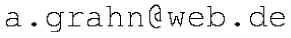
\includegraphics[height=2.7ex]{mailto}}
\maketitle

\begin{abstract}\noindent
A \LaTeX{} package for embedding interactive Adobe Flash (SWF) and 3D files (Adobe U3D \& PRC) as well as video and sound files or streams (FLV, MP4/H.246, MP3) into PDF documents with Adobe Reader-9/X compatibility.\\[0.2\baselineskip]
\begin{sloppypar}\foreignlanguage{nohyphenation}{\noindent\emph{Keywords}: \keywords}\end{sloppypar}
\end{abstract}

\tableofcontents

\section{Introduction}
This package provides an interface to embed, in the first place, interactive Flash (SWF) and 3D objects (Adobe U3D \& PRC) into PDF documents. Video and sound files or streams in the popular MP4, FLV and MP3 formats can be embedded as well. However, a media player Flash component is required for playback, as will be explained shortly. Playback of multimedia files uses Adobe Flash Player, which was bundled with Adobe Reader 9 and 10 versions. Unfortunately, beginning with Adobe Reader 11, it must be installed as a separate plug-in.

Among the supported media types, video and sound files require an additional Flash (SWF) application for playback, which must be either embedded into the PDF or loaded at runtime from the internet. There are numerous such players, both open-source and commercial, available on the internet. One of them is the highly configurable open-source `StrobeMediaPlayback.swf'~\cite{strobe}, maintained by Adobe and hosted on \href{http://sourceforge.net/projects/osmf.adobe/files/}{SourceForge.net}. Package `media9' comes with an enhanced version of `StrobeMediaPlayback.swf'. In addition, two simple players for video and audio, `VPlayer.swf' and `APlayer.swf' are included, which can be used instead. They provide sufficient functionality for playing embedded files and streamed media.

Flash Player supports the efficient H.264 codec for video compression. MP4/H.264 video files can be encoded from existing video files and from numbered bitmap sequences using the \verb+ffmpeg+ command line tool (\url{http://ffmpeg.org}). In order to allow for precise seeking within video files it is necessary to encode them with a sufficient number of key frames. The command line for recoding an existing video file \verb+video.avi+ into \verb+video.mp4+ reads
\begin{Verbatim}
  ffmpeg -i video.avi -vcodec libx264 -x264opts keyint=30 -r 30 video.mp4
\end{Verbatim}
From a sequence \verb+frame-0.png+, \verb+frame-1.png+, ... of bitmap files, an MP4 video is produced by
\begin{Verbatim}
  ffmpeg -i frame-%d.png -vcodec libx264 -x264opts keyint=30 -r 30 video.mp4
\end{Verbatim}
Both examples insert a key frame at every second since the frame rate is set to 30 fps.

\emph{Note:} `media9' package replaces the now obsolete `movie15' package. `media9' is based on the RichMedia Annotation (Annotations are the interactive elements in a document, in PDF specification parlance.), an Adobe addition to the PDF specification~\cite{supplement}, while `movie15' uses the old multimedia framework (`Screen Annotation') of pre-9 Readers which depends on third-party plug-ins and which does not support recent media file formats.

Package `media9' supports the usual PDF making workflows, i.\,e. pdf\LaTeX{}, Lua\LaTeX, \LaTeX{} $\rightarrow$ \verb+dvips+ $\rightarrow$ \verb+ps2pdf+/Distiller and \pXepLaTeX{} $\rightarrow$ \verb+(x)dvipdfmx+.

The final PDF can be viewed in current Adobe Readers on MS Windows and other platforms. On Unix platforms including Linux, however, support of Flash, video and sound was discontinued at Reader version 9.4.2, probably for security reasons. On tablets and phones running Android or iOS, ezPDF Reader was reported to play video and sound files embedded with `media9'.

\section{Requirements}
\begin{trivlist}
\makeatletter
\item l3kernel (\LaTeX{} package), version $\ge \g@mix@liiikerneldate$
\item l3packages (\LaTeX{} package), version $\ge \g@mix@liiipkgdate$
\makeatother
\item pdf\TeX{}, version $\ge1.30$
\item Ghostscript, version $\ge8.31$ or Adobe Distiller for PS to PDF conversion
\item dvipdfmx, version $\ge 20120420$ for DVI to PDF conversion
\item Adobe Reader, version $\ge9$
\end{trivlist}

\section{Installation}
MiK\TeX{} and \TeX{}Live users should run the package manager for installation and updates.

Otherwise, a manual installation into the \emph{local} TeX-Directory-Structure (TDS) root directory is done along the following steps:
\begin{enumerate}
  \item Download the TDS compliant package file `\href{http://tug.ctan.org/tex-archive/install/macros/latex/contrib/media9.tds.zip}{media9.tds.zip}' from CTAN.
  \item Find the local TDS root directory by running\\
  {\tt\phantom{xx}kpsewhich -var-value TEXMFLOCAL}\\
  on the command line. The local TDS root directory is intended for packages that are not maintained by the \TeX{}Live package manager.
  \item Unzip `\href{http://tug.ctan.org/tex-archive/install/macros/latex/contrib/media9.tds.zip}{media9.tds.zip}' into the local TDS root directory previously found. Depending on the location of this directory, you may need to be logged in as Root/Administrator.
  \item After installation, update the filename database by running `{\tt texhash}' on the command line. Again, Root/Administrator privileges may be required.
\end{enumerate}
For updating the package, repeat the steps given above.

\section{Using the package}\label{pkguse}
Invoke the package by putting the line
\begin{verbatim}
    \usepackage[<package options>]{media9}
\end{verbatim}
to the preamble of your document, i.\,e. somewhere between \verb+\documentclass+ and \verb+\begin{document}+.

`media9' honours the package options:
\begin{verbatim}
dvipdfmx
xetex
bigfiles
draft
final
activate=...
deactivate=...
windowed=...
transparent
passcontext
3Dplaytype=...
3Dplaycount=...
3Dplayspeed=...
3Dtoolbar
3Dnavpane
3Dpartsattrs=...
3Dmenu
3Dbg=...
3Dlights=...
3Drender=...
\end{verbatim}
Except for `\verb+dvipdfmx+', `\verb+xetex+' and `\verb+bigfiles+', the options above are also available (among others) as command options and will be explained shortly. However, if used as package options they have global scope, taking effect on all embedded media in the document. In turn, command options locally override global settings. Options without an argument are boolean options and can be negated by appending `\verb+=false+'.

\XeLaTeX{} will be auto-detected. Therefore package option `\verb+xetex+' is optional. However, in the case of  \verb+dvipdfmx+, package option `\verb+dvipdfmx+' is mandatory because it cannot be auto-detected.

\begin{animateinline}[autoplay,loop]{1.5}\strut\emph{Important:}\newframe\newframe[5]\end{animateinline} If PDF is generated via DVI and Postscript by the command sequence \verb+latex+ $\rightarrow$ \verb+dvips+ $\rightarrow$ \verb+ps2pdf+, \verb+dvips+ option `\verb+-Ppdf+' should \emph{not} be set when converting the intermediate DVI into Postscript. If you cannot do without, put `\verb+-D 1200+' \emph{after} `\verb+-Ppdf+' on the command line. Users of \LaTeX-aware text editors with menu-driven toolchain invocation, such as \TeX{}nicCenter, should check the configuration of the \verb+dvips+ call.

Option `\verb+bigfiles+' is only relevant for the \verb+latex+ $\rightarrow$ \verb+dvips+ $\rightarrow$ \verb+ps2pdf+ workflow. It may be needed if large media files cause \verb+latex+ to abort with error `\verb+TeX capacity exceeded+'. See Sect.\ \ref{bugs}.

\section{The user interface}
Package `media9' provides commands for media inclusion (\verb+\includemedia+) and insertion of media control buttons (\verb+\mediabutton+). The latter is introduced in Sect. \ref{mbtn}.

\subsection{Media inclusion}
\begin{verbatim}
\includemedia[<options>]{<poster text>}{
    <main Flash (SWF) file or URL  |  3D (PRC, U3D) file>}
\end{verbatim}

The last argument, \verb+<main Flash (SWF) file or URL | 3D (PRC, U3D) file>+, is the main interactive application to be inserted into the PDF. In the case of Flash, this can be a local SWF file, or a URL, such as a YouTube video player. A local file will become part of the final PDF file, while Flash content from a URL requires an internet connection when the user activates it in Adobe Reader. A URL must be fully qualified, i.\,e., starting with either `\verb+http[s]://+' or `\verb+ftp://+'. As for 3D content, Adobe Reader only supports U3D or PRC files embedded in the PDF; they cannot be loaded or streamed during runtime. The most frequent use of \verb+\includemedia+ will likely be embedding video or sound files for playback in Adobe Reader. For this we need some media player, which is an SWF file we embed as our main application. It will be configured to load, upon activation, a particular video or sound file that was embedded as a resource into the PDF or is to be streamed from the internet. This will be shown later. Note that a local file (main application or resource) will only once be physically embedded in order to keep the final PDF file size small. If the same file (identified by MD5 checksum) appears in other \verb+\includemedia+ commands, only a reference will be inserted that points to the same storage location in the PDF.

Argument \verb+<poster text>+ defines the size of the rectangular region of the document page in which the media will be displayed. Moreover, \verb+<poster text>+ will be shown in case the media has not been activated.
%(Internally, \verb+<poster text>+ is put into a \LaTeX{} box, which is used as the appearance of the PDF annotation, i.\,e. the interactive region created by \verb+\includemedia+, in PDF specification parlance.)
\verb+<poster text>+ can be anything that \LaTeX{} can typeset, such as an \verb+\includegraphics+ command serving as a poster image, a PGF/TikZ/PSTricks inline graphics or just ordinary text. Alternatively, \verb+<poster text>+ can be left blank in which case the size of the media rectangle should be set with options `\verb+width+', `\verb+height+' and optionally with `\verb+depth+'. If sizing options `\verb+width+' and `\verb+height+' are given \emph{together} with \verb+<poster text>+, \verb+<poster text>+ will be shrunk or stretched to fit exactly into the rectangle defined by the options, possibly changing the original aspect ratio of the poster text. On the other hand, if only one of `\verb+width+' or `\verb+height+' is given, the other dimension of \verb+<poster text>+ is scaled such that the original aspect ratio is preserved.

A list of directories where \TeX{} searches for media and resource files can be set-up by means of
\begin{verbatim}
\addmediapath{<directory>}
\end{verbatim}
This command appends one directory at a time to the search list. To specify more directories, just use it repeatedly. The path separator is always `\verb+/+', independent from the operating system.

The following section explains all command options provided. They are passed to the media inclusion command as a comma separated list enclosed in a pair of square brackets.

\subsection{Command options}
A subset of the command options (see Sect. \ref{pkguse}) can also be used as package options, which lets them apply to all embedded media. Some of the options listed here are meaningful only for a specific media type (either Flash or 3D), which will be noted explicitly if not obvious. Dedicated sections covering Flash, video and sound as well as 3D inclusion will follow later on in this document.

\begin{verbatim}
width=<width>,
height=<height>,
depth=<depth>
\end{verbatim}
Resize the media playback area, overriding the original dimensions of the {\tt<poster text>} argument. Option `\verb+depth+' specifies how far the playback area should extend below the base line of the running text. If only one of `\verb+width+' or `\verb+height+' is given, the other dimension is scaled to maintain the aspect ratio of \verb+<poster text>+. Any valid \TeX{} dimension is accepted as a parameter. In addition, the length commands \verb+\width+, \verb+\height+, \verb+\depth+ and \verb+\totalheight+ can be used to refer to the original dimensions of \verb+<poster text>+.
\begin{verbatim}
label=<label key>
\end{verbatim}
The media annotation is given a label, \verb+<label key>+, which should be unique. Labelled media annotations can be targeted by the media actions of a control button (see description of the \verb+\mediabutton+ command in Sect. ~\ref{mbtn}). Moreover, a reference to the RichMedia Annotation object (of type `\verb+AnnotRichMedia+') is assigned to the JavaScript variable \verb+annotRM['<label key>']+ in order to facilitate its access in JavaScript. Note that the JavaScript reference is known only after the first opening of the page containing the media.
\begin{verbatim}
scale=<factor>
\end{verbatim}
Scales the playback area by \verb+<factor>+.
\begin{verbatim}
addresource=<local file>,
addresource=<another local file>,
...
\end{verbatim}
Every invocation of this option embeds another local file that is required to run the main Flash application or 3D file (last argument of \verb+\includemedia+). Typically, this option is used to embed video files, media player skins, XML files (such as databases), additional objects to appear in a 3D scene etc. If an already embedded file is needed in another \verb+\includemedia+ command, this option must be given there again. However, the file in question will only once be physically embedded in order to keep the PDF file small.
\begin{verbatim}
flashvars={<some_var=some_val&another_var=another_val&...>}
\end{verbatim}
(Flash only) Usually, Flash applications can be configured via ActionScript (AS) variables the programmer of the application has made visible from outside. A typical use would be to set the video source of a media player to point to an embedded MP4 file or to a live stream, or to set the speaker volume for playback of an MP3 file. The argument of the \verb+flashvars+ option is a list of \verb+<AS variable>=<value>+ pairs separated by `\verb+&+' and enclosed in a pair of braces (\verb+{...}+).

Note: If a variable is to be set to point to an embedded resource, the value of the variable must be given in exactly the same way as with the `\verb+addresource+' option. Otherwise the name of the embedded file cannot be resolved. For example,
\begin{verbatim}
  addresource=path/to/video.mp4
\end{verbatim}
implies
\begin{verbatim}
  flashvars={vid=path/to/video.mp4&...}
\end{verbatim}
if, for a particular media player, the video source is set through ActionScript variable `\verb+vid+'.

(Note for 3D) Resource files used in 3D scenes cannot be loaded by means of ActionScript variables. This must be done by 3D JavaScript during activation of the 3D scene in the Reader. 3D JavaScript can be attached using option `\verb+add3Djscript+', see below.
\begin{verbatim}
activate=onclick | pageopen | pagevisible
\end{verbatim}
Decides on how to activate the media annotation. `\verb+activate=onclick+' is default behaviour and does not need be given explicitly; embedded media is activated when the user clicks on it or by a JavaScript. It is recommended to provide a poster image with the \verb+<poster text>+ argument in that case. `\verb+pageopen+' and `\verb+pagevisible+' automatically activate the media when the page becomes visible; `{\tt pagevisible}' is better for two-up and continuous page display.
\begin{verbatim}
deactivate=onclick | pageclose | pageinvisible
\end{verbatim}
Decides on how to de-activate the media annotation. `\verb+deactivate=pageclose+' is default behaviour and does not need be given explicitly; media is automatically de-activated when the user leaves the page containing the media. `\verb+pageinvisible+' is similar, but may be better for two-up and continuous page display. Setting `\verb+deactivate=onclick+' requires user interaction for de-activating the media, either by right-click and chosing `\emph{\sffamily Disable Content}' or by a JavaScript.
\hypertarget{draftfinal}{}%
\begin{verbatim}
draft
final
\end{verbatim}
With `\verb+draft+' the media is not embedded. Instead, a box is inserted that has the dimensions of \verb+<poster text>+, subject to the resizing options `\verb+width+', `\verb+height+', `\verb+depth+' and `\verb+scale+'. Option `\verb+final+' does the opposite as it forces the media to be embedded. Both options can be used to reduce compilation time during authoring of a document. To get the most out of them it is recommended to set `\verb+draft+' globally as a package or class option and to set `\verb+final+' locally as a command option of the media annotation that is currently worked on. After the document has been finished, the global `\verb+draft+' option can be removed.
\begin{verbatim}
windowed[= false | [<width>x<height>][@<position>] ]
\end{verbatim}
The media is played in a floating window, instead of being played in an embedded fashion. The floating window size is specified via the optional argument \verb+<width>x<height>+, where \verb+<width>+ and \verb+<height>+ are given in pixels (integer numbers without unit). If the size is not given, a default size is guessed from the annotation size. Optionally, the position of the floating window on the screen can be specified through \verb+@<position>+, where \verb+<position>+ may assume one of `\verb+tl+', `\verb+cl+', `\verb+bl+', `\verb+bc+', `\verb+br+', `\verb+cr+', `\verb+tr+', `\verb+tc+' or `\verb+cc+'. The position specifiers have the following meaning:\quad{\fboxsep=1pt\fbox{\vtop{\hbox{\ttfamily\fbox{\rule{0pt}{1.5ex}tl} \fbox{\rule{0pt}{1.5ex}tc} \fbox{\rule{0pt}{1.5ex}tr}} \hbox{\ttfamily\fbox{\rule{0pt}{1.5ex}cl} \fbox{\rule{0pt}{1.5ex}cc} \fbox{\rule{0pt}{1.5ex}cr}} \hbox{\ttfamily\fbox{\rule{0pt}{1.5ex}bl} \fbox{\rule{0pt}{1.5ex}bc} \fbox{\rule{0pt}{1.5ex}br}}}}}\\[0.5ex]
Default window position is `\verb+cc+', that is, centred on the screen. `\verb+false+' can be set to override a global setting via package options.
\begin{verbatim}
transparent
\end{verbatim}
Indicates whether underlying page content is visible through transparent areas of the embedded media. Default is `\verb+transparent=false+'; media artwork is drawn over an opaque background prior to composition over the page content.
\begin{verbatim}
passcontext
\end{verbatim}
(Flash only) If set, user right-clicks are passed through to the context menu of the embedded Flash application, replacing the default Adobe Reader context menu. Useful for cases where the Flash programmer provided additional functionality through the context menu of his application.
\begin{verbatim}
3Dtoolbar
\end{verbatim}
Indicates whether a 3D toolbar should be shown in the Reader on top of the embedded 3D model.
\begin{verbatim}
3Dnavpane
\end{verbatim}
If set, the 3D navigation pane displaying the 3D Model Tree becomes visible in the Reader when the content is initially activated.
\begin{verbatim}
3Dcoo=<x> <y> <z>
\end{verbatim}
\verb+<x> <y> <z>+ specify the positional vector $\overrightarrow{COO}$ of the centre of orbit of the virtual camera. Real numbers in fixed and floating point notation are accepted.
\begin{verbatim}
3Dc2c=<x> <y> <z>
\end{verbatim}
\verb+<x> <y> <z>+ specify a direction vector $\overrightarrow{C2C}$ of arbitrary length, originating in the centre of orbit and pointing to the virtual camera. Real numbers in fixed and floating point notation are accepted.
\begin{verbatim}
3Droll=<roll>
\end{verbatim}
Prescribes an initial camera roll around the optical axis (in clockwise direction, if \verb+<roll>+ is greater that zero); measured in degrees and given as fixed or floating point real number.
\begin{verbatim}
3Dc2w=<12 element camera-to-world matrix>
\end{verbatim}
This option directly sets the camera-to-world transformation matrix according to the PDF specification. This is an expert option to be used \emph{instead} of the `\verb+3Dc2c+', `\verb+3Dcoo+' and `\verb+3Droll+' options. Only fixed point real numbers are accepted.
\begin{verbatim}
3Dpsob=Min | Max | W | H
\end{verbatim}
Expert option which directly sets either the \verb+/PS+ entry in the case of perspective projection or the \verb+/OB+ entry in the case of orthographic projection to one of the four possible values. Default value is \verb+Min+.
\begin{verbatim}
3Droo=<r>
\end{verbatim}
\verb+<r>+ is a positive fixed or floating point number specifying the radius of orbit $ROO$ of the virtual camera. Good values can be found by means of the `\verb+3Dmenu+' option.
\begin{verbatim}
3Daac=<angle>
\end{verbatim}
This option sets the aperture angle of the camera, measured in degrees, for the perspective view mode. Fixed and floating point real numbers between 0 and 180 are admissible. A sensible value of 30 is pre-set by default. Larger values can be used to achieve wide-angle or fish-eye effects. See example~\ref{u3dex} in section~\ref{sec:3Dintro}. This option excludes the use of the `\verb+3Dortho+' option.
\begin{verbatim}
3Dortho[=<orthographic scaling factor>]
\end{verbatim}
Switches from the default perspective to orthographic view mode. In orthographic view, the 3D object is parallelly projected onto the virtual camera chip. The projected image is scaled by \verb+<orthographic scaling factor>+ before reaching the camera chip; default value is 1. The optimal value for the scaling factor is given by $1/D$, where $D$ is the diameter of the smallest enclosing sphere of the 3D object in World coordinate units. Fixed and floating point real numbers are accepted. The camera should be positioned outside the 3D object. For this, the radius of orbit (option `\verb+3Droo+') should be greater than $D/2$. Good values for orthographic scaling and orbital radius can easily be found by means of the `\verb+3Dmenu+' option. Option `\verb+3Dortho+' excludes the use of the `\verb+3Daac+' option.
\hypertarget{3dmenu}{}%
\begin{verbatim}
3Dmenu
\end{verbatim}
Mainly used during document authoring. Adds three entries, `\emph{\sffamily Generate Default View}', `\emph{\sffamily Get Current View}' and `\emph{\sffamily Cross Section}' to the context (right-click) menu of an activated 3D annotation. Moreover, it allows individual parts of the scene to be scaled, translated and rotated against the remaining scene objects using the keyboard. Their new position can be saved in the current view. Parts to be modified should be highlighted with the mouse first (the part's bounding box becomes visible). Then, arrow keys \keys{\arrowkeyleft}, \keys{\arrowkeyright} let the part spin around its vertical axis, and \keys{\arrowkeyup}, \keys{\arrowkeydown} tilt against the vertical position. \keys{X}, \keys{\shift+X}, \keys{Y}, \keys{\shift+Y}, \keys{Z}, \keys{\shift+Z} translate the selected part along the World axes and \keys{S}, \keys{\shift+S} scale the part.

`\emph{\sffamily Generate Default View}' computes optimal camera settings such that the visible parts of the 3D scene fit tightly into the viewing area. The result is printed, formatted as a list of \verb+\includemedia+ options, into the JavaScript console. The calculation is based on the 3D object size and its position in the World coordinate system as well as the current viewing mode (perspective or orthographic).

`\emph{\sffamily Cross Section}' is a toggle switch to add or remove a cross section to or from the current view. If a part of the 3D scene was previously selected, the central rotating point of the section plane is put into the part's centre, otherwise into the target point of the camera. The section plane can be rotated around the vertical axis and tilted against its upright position using the arrow keys \keys{\arrowkeyleft}, \keys{\arrowkeyright}, \keys{\arrowkeyup} and \keys{\arrowkeydown}. Keys \keys{X}, \keys{\shift+X}, \keys{Y}, \keys{\shift+Y}, \keys{Z}, \keys{\shift+Z} move the section plane along the World axes.

`\emph{\sffamily Get Current View}' writes camera settings, any part alterations, an optional cross section as well as part and scene rendering attributes of the current view into the JavaScript console. The output is a readily formatted \verb+VIEW+ section to be inserted into or appended to a file of predefined views. See option `\verb+3Dviews+'. All settings reachable via the `\emph{\sffamily Part Options}' and `\emph{\sffamily Viewing Options}' context menu items are written to the \verb+VIEW+ section.
\begin{verbatim}
3Dbg=<r> <g> <b>
\end{verbatim}
This option sets the background colour of the 3D scene. Only fixed point real numbers in the range from 0 to 1 are allowed for the colour components. Option `\verb+transparent+' may not be set at the same time.
\begin{verbatim}
3Dlights=<lighting scheme>
\end{verbatim}
Sets the default lighting scheme. The following values are honoured: `\verb+None+', `\verb+White+', `\verb+Day+', `\verb+Night+', `\verb+Hard+', `\verb+Primary+', `\verb+Blue+', `\verb+Red+', `\verb+Cube+', `\verb+CAD+', `\verb+HeadLamp+'. The default is to use the lighting scheme as specified within the 3D artwork.
\begin{verbatim}
3Drender=<render mode>
\end{verbatim}
\begin{flushleft}
Sets the default render mode. The following values are honoured: `\verb+Solid+', `\verb+SolidWireframe+', `\verb+Transparent+', `\verb+TransparentWireframe+', `\verb+BoundingBox+', `\verb+TransparentBoundingBox+', `\verb+TransparentBoundingBoxOutline+', `\verb+Wireframe+', `\verb+ShadedWireframe+', `\verb+HiddenWireframe+', `\verb+Vertices+', `\verb+ShadedVertices+', `\verb+SolidOutline+', `\verb+Illustration+', `\verb+ShadedIllustration+'.
\end{flushleft}
\begin{verbatim}
3Dpartsattrs=restore | keep
\end{verbatim}
When the user selects another view from the list of predefined views (see option `\verb+3Dviews+'), attributes of individual parts, such as opacity, visibility, render mode,
translation in space,
which all can be set from within the Reader or by means of a file of predefined views, are reset to their original states as defined in the embedded 3D file, before any new part settings are applied. This default behaviour can be overridden by `\verb+3Dpartsattrs=keep+'. This will preserve current part attributes when the user selects another predefined 3D view in the Reader.
\hypertarget{3Dviews}{}%
\begin{verbatim}
3Dviews=<views file>
\end{verbatim}
Instead of or in addition to the default view (options `\verb+3Dcoo+', `\verb+3Dc2c+', `\verb+3Droll+', `\verb+3Droo+', `\verb+3Daac+', `\verb+3Dortho+'), further \emph{named views} can be predefined in an auxiliary file \verb+<views file>+. Besides the virtual camera position, it is possible to adjust the rendering attributes, such as visibility and transparency, as well as position and scaling of every single part in the 3D scene. Moreover, background colour and scene lighting can be set individually for every view. The additional views can later be selected either from a drop down list in the tool bar that is associated with the activated 3D object in the Reader or from the context menu of the 3D object.

The file \verb+<views file>+ is structured into view sections, one for every view:
\begin{verbatim}
  VIEW[=<optional name>]
    COO=<x> <y> <z>
    C2C=<x> <y> <z>
    ROLL=<roll>
  %  C2W=<camera-to-world matrix> % instead of COO, C2C and ROLL
    ROO=<roo>
    AAC=<aac>
  %  ORTHO[=<othographic scaling factor>] % instead of AAC
    BGCOLOR=<r> <g> <b>
    RENDERMODE=<render mode>
    LIGHTS=<lighting scheme>
    CROSSSECT
      CENTER=<x> <y> <z>
      NORMAL=<x> <y> <z>
    END
    PARTSATTRS=keep
    PART=<part name  as in the Model Tree (required, optional if UTF16NAME present)>
      UTF16NAME=<part name as hex encoded Unicode string>
      VISIBLE=true | false
      OPACITY=<part opacity>
      RENDERMODE=<part render mode>
      TRANSFORM=<12 element transformation matrix>
    END
    PART=<...>
      ...
    END
    etc.
  END

  VIEW
    ...
  END

  etc.
\end{verbatim}
A view section starts with the keyword \verb+VIEW+, optionally followed by a name for the view, and ends with the keyword \verb+END+. If no name is given to the view, a default one is created, consisting of `View' followed by the number of the current \verb+VIEW+ section in the file. A \verb+VIEW+ section may contain optional entries for setting the camera position and global rendering attributes of the scene, a \verb+CROSSSECT+ subsection as well as \verb+PART+ subsections for setting rendering and other attributes of parts individually. Table~\ref{tab:views} lists the entries in a \verb+VIEW+ section.

Part sub-sections are opened by \verb+PART=<part name>+ and closed by \verb+END+. There may be as many part subsections as there are parts in a 3D scene. Table~\ref{tab:parts} lists the possible entries in a \verb+PART+ sub-section. All entries are optional. However, a \verb+UTF16NAME+ entry is recommended, as the part name may contain non-ASCII characters. The value of the \verb+UTF16NAME+ key is the part name as a hex-encoded Unicode string. If \verb+UTF16NAME+ is not used, the part name in the 3D file must be entirely composed of ASCII characters. In that case, \verb+<part name>+ is mandatory and must match the part name as indicated in the Model Tree of the 3D object (accessible via right-click onto the model in the Reader). The part can be scaled and repositioned by means of a \verb+TRANSFORM+ entry which takes a 12-element transformation matrix as its value. Remaining entries in a part sub-section control the visual appearance of the part.

A view section may contain at most one \verb+CROSSSECT+ sub-section. It inserts a section plane at a definite position and orientation in the 3D space, controlled by optional \verb+CENTER+ and \verb+NORMAL+ entries. See Table~\ref{tab:crosss} for explanation.

The views file can be commented. As usual, comments start with the percent sign.

To facilitate the creation of a views file, option `\verb+3Dmenu+' can be added to \verb+\includemedia+ (see above). It creates context (right-click) menu entry `Get Current View' which outputs a complete \verb+VIEW+ section corresponding to the current view of the 3D object in the Reader, including camera position, an optional cross section, and all part and viewing options that can be modified via the 3D toolbar (option `\verb+3Dtoolbar+') or the context menu of the 3D object (entries `\emph{\sffamily Part Options}', `\emph{\sffamily Viewing Options}'). Hence, apart from tweaking one or another entry, there should be no need for writing views files by hand.
\begin{verbatim}
3Dplaytype=linear | oscillating
\end{verbatim}
According to the PDF specification, embedded keyframe animations can be played in two ways. If set to `\verb+linear+', keyframe animations are driven linearly from beginning to end, while `\verb+oscillating+' lets the animation play in a forth-and-back manner.
\begin{verbatim}
3Dplaycount=<integer number>
\end{verbatim}
A non-negative \verb+<integer number>+ represents the number of times the animation is played. A negative integer indicates that the animation is infinitely repeated. This value is ignored if option \verb+3Dplaytype+ is not set.
\begin{verbatim}
3Dplayspeed=<positive number>
\end{verbatim}
This option can be used to adjust the keyframe animation speed. A value of `1' corresponds to the default speed defined in the 3D file.
\hypertarget{add3Djscript}{}%
\begin{verbatim}
add3Djscript=<3D JavaScript file>,
add3Djscript=<another 3D JavaScript file>,
...
\end{verbatim}
Things like animation, lighting, background of 3D objects etc. may also be script driven. Every invocation of `\verb+add3Djscript+' associates another JavaScript file with the 3D object. Upon activation of the 3D object, the scripts are executed once in the order of their inclusion. Refer to the Acrobat 3D JavaScript Reference~\cite{jscript3D} for syntax details. The following 3D JavaScript loads an image file that was attached by `\verb+addresource=images/sunset.jpg+' and uses it as the scene background.
\begin{verbatim}
  sunset = new Image(new Resource('pdf://images/sunset.jpg'));
  reh = new RenderEventHandler();
  reh.onEvent = function(event) {
    runtime.removeEventHandler(this);
    event.canvas.background.image=sunset;
  }
  runtime.addEventHandler(reh);
\end{verbatim}
\hypertarget{3dscripts}{}For convenience, subdirectory `javascript' of the `media9' installation contains three 3D JavaScript files which may come in handy at times: `animation.js' enables embedded keyframe animation in 3D files; `3Dspintool.js' enables the Spin tool of the 3D plugin for easier rotating the 3D object with the mouse; `asylabels.js' adds `billboard behaviour' to text labels in Asymptote ($\ge v2.17$) generated PRC files for improved visibility; text labels always face the camera while rotating the 3D object with the mouse.

\begin{table}[bp]%[p]%[htbp]
  \centering
  \caption{Entries in a {\tt VIEW} section.}\label{tab:views}
  \begin{tabular}[t]{p{0.24\linewidth}lp{0.4\linewidth}}\hline
  key & type & remarks\\\hline\hline
  {\tt COO} & three numbers & centre of orbit, see option `{\tt 3Dcoo}'\\
  {\tt C2C} & three numbers & centre of orbit to camera vector, see option `{\tt 3Dc2c}'\\
  {\tt ROO} & number & radius of orbit, see option `{\tt 3Droo}'\\
  {\tt C2W} & 12 numbers & camera-to-world transformation matrix, see option `{\tt 3Dc2w}'\\
  {\tt AAC} & number & camera aperture angle, see option `{\tt 3Daac}'\\
  {\tt ORTHO} & number (optional) & enables orthographic view, see option `{\tt 3Dortho}'\\
  {\tt PSOB} & string & expert setting, see option `{\tt 3Dpsob}'\\
  {\tt ROLL} & number & camera roll, see option `{\tt 3Droll}'\\
  {\tt BGCOLOR} & three numbers & 3D scene background colour (RGB), see option `{\tt 3Dbg}'\\
  {\tt RENDERMODE} & string & render mode of the 3D object, see option `{\tt 3Drender}'\\
  {\tt LIGHTS} & string & lighting scheme, see option `{\tt 3Dlights}'\\
  {\tt PARTSATTRS} & string & allowed values are `{\tt keep}' and `{\tt restore}'; decides on whether to restore or not original part attributes before applying new ones from this view; see option `{\tt 3Dpartsattrs}'\\
  {\tt PART}\,\,(sub-sec\-tion) & string & part name as in the model tree; optional if a {\tt UTF16NAME} entry is present in the sub-section opened by a {\tt PART} keyword, otherwise required; see Table~\ref{tab:parts} for list of possible entries\\
  {\tt CROSSSECT}~(sub-section) & -- & see Table~\ref{tab:crosss} for list of possible entries\\
  \hline
  \end{tabular}
\end{table}

\begin{table}%[p]%[htbp]
  \centering
  \caption{Entries in a {\tt PART} sub-section.}\label{tab:parts}
  \begin{tabular}[t]{llp{0.5\linewidth}}\hline
  key & type & remarks\\\hline\hline
  {\tt UTF16NAME} & hex string & part name in UTF-16 (aka Unicode), encoded as a hexadecimal string; optional, but useful for part names composed of non-latin characters;\\
  {\tt VISIBLE} & boolean & a flag (`{\tt true}' or `{\tt false}') indicating the visibility of this part\\
  {\tt OPACITY} & number & a number between 0.0 and 1.0 specifying the opacity of this part\\
  {\tt RENDERMODE} & string & rendermode of this part, overrides global {\tt RENDERMODE} value in parent {\tt VIEW} section, see option `{\tt 3Drender}'\\
  {\tt TRANSFORM} & 12 numbers & transformation matrix defining the part's position and scaling\\
  \hline
  \end{tabular}
\end{table}

\begin{table}%[p]%[htbp]
  \centering
  \caption{Entries in a {\tt CROSSSECT} sub-section.}\label{tab:crosss}
  \begin{tabular}[t]{llp{0.5\linewidth}}\hline
  key & type & remarks\\\hline\hline
  {\tt CENTER} & three numbers & central point coordinates of the section plane\\
  {\tt NORMAL} & three numbers & normal vector coordinates of the section plane pointing into the cut-off region\\
  \hline
  \end{tabular}
\end{table}

\clearpage
\subsection{Control buttons}\label{mbtn}
\begin{verbatim}
\mediabutton[<options>]{<normal button text or graphic>}
\end{verbatim}
This command inserts a clickable button for media control. Actions to be performed are specified through options `\verb+mediacommand+', `\verb+3Dgotoview+' and `\verb+jsaction+'. By using these options repeatedly and in any combination, several actions can be bound to one media button, and one media button can be used to control several media at the same time. Media actions are started in the given order but performed in parallel, because they do not wait for each other to finish. The target of an action is specified via the label key that was also given to a particular media by the `\verb+label+' option of `\verb+\includemedia+'. Individual button faces can be defined for the `mouse-over' and `mouse-button-down' events using the `\verb+overface+' and `\verb+downface+' options. Without options, the button produced does nothing. The options provided are as follows:
\begin{verbatim}
overface=<mouse-over text or graphic>
\end{verbatim}
If specified, the media button changes its appearance when the mouse pointer is moved over it. Without this option, the button appearance does not change. An \verb+\includegraphics+ command may need to be enclosed in braces.
\begin{verbatim}
downface=<mouse-button-down text or graphic>
\end{verbatim}
If specified, the media button changes its appearance when the mouse button is pressed while the pointer is over it. When pressed, the button is always slightly offset to appear as if it were being pushed below the surface of the page. An \verb+\includegraphics+ command may need to be enclosed in braces.
\begin{verbatim}
3Dgotoview=<label key>[:<view specification>]
\end{verbatim}
Selects a view from the list of predefined views associated with a 3D media inclusion (see option `\verb+3Dviews+'). The target media is specified by \verb+<label key>+, as defined by the `\verb+label+' option of `\verb+\includemedia+'. \verb+<label key>+ alone without a view specification simply activates the 3D object if not yet activated. {\tt<view specification>} which is separated from the label key by a colon (\verb+:+) can be one of the following: an integer specifying the zero-based index into the list of views in the 3D views file; one of `\verb+D+', `\verb+F+', `\verb+L+', `\verb+N+', `\verb+P+' indicating the default, first, last, next or previous view in the list of views; a string delimited by `\verb+(+' and `\verb+)+' matching the name of a view as specified by the `\verb+VIEW=...+' entry in the views file. The option can be given several times to simultaneously change the view in more than one 3D inclusion. However, it cannot be used to create an animation effect within the same 3D inclusion, because \verb+3Dgotoview+ actions are executed in parallel.
%For this, one may implement a 3D JavaScript function that is associated with the media button using the `\verb+mediacommand+' option.
\begin{verbatim}
mediacommand=<label key>[:<command> [<arg1> <arg2> ...]]
\end{verbatim}
A media command \verb+<command>+, with arguments if required, is sent to a media inclusion identified by \verb+<label key>+, as defined by the `\verb+label+' option of `\verb+\includemedia+'. \verb+<label key>+ alone without a command specification simply activates the media, if not yet activated. The option can be multiply used within the same button to target different media inclusions at the same time or to execute several commands for the same media. Depending on the type of the target media (3D or Flash), \verb+<command>+ is either the name of a JavaScript function defined in a 3D JavaScript file associated with the 3D media (see option `\verb+add3Djscript+') or the name of an ActionScript function that was exposed by the embedded Flash file. ActionScript functions are exposed to the scripting context of the hosting document by using the \verb+ExternalInterface+ call within the Flash file. Arguments to be passed to \verb+<command>+ must be separated by spaces and the whole list be enclosed in `\verb+[+' and `\verb+]+'. Arguments can be of Boolean type (\verb+true+, \verb+false+), numbers (integer, reals) and strings. String arguments must be passed as \verb+(string arg)+, i.\,e. enclosed in parentheses, while numbers and Booleans are passed as they are. Of course, the number of arguments and their types must match the definition of the function to be called. Media players VPlayer.swf and APlayer.swf shipping with media9 expose a number of ActionScript functions that can be used with this option (see Tab. \ref{AVPlayerMethods}). \verb+<command> [<arg1> <arg2> ...]+ must be enclosed in braces if there are embedded equals signs or commas.
\begin{verbatim}
jsaction=[<label key>:]{<JavaScript code>}
\end{verbatim}
The JavaScript code is executed in the context of the document's instance of the JavaScript engine (there is one instance of the JavaScript engine per open document in Adobe Reader). \verb+<JavaScript code>+ is required and must be enclosed in braces. Unlike media actions defined with options `\verb+mediacommand+' and `\verb+3Dgotoview+', the JavaScript action defined here is not targeted at a particular embedded media and can be used to run arbitrary code. Therefore, \verb+<label key>+ is optional. If provided, it must be separated from \verb+<JavaScript code>+ by a colon. However, it is recommended to provide a label key. It ensures that \verb+annotRM['<label key>']+ is a valid JavaScript reference to the \verb+AnnotRichMedia+ object. \verb+annotRM['<label key>']+ can be used to get access to the global context of the annotation's instance of the 3D JavaScript engine (there is one instance of the 3D JavaScript engine per activated RichMedia Annotation with 3D content). The 3D JavaScript context of a 3D model can be accessed as \verb+annotRM['<label key>'].context3D+. Refer to the Acrobat 3D JavaScript Reference~\cite{jscript3D} for details on built-in JavaScript objects that are available in the 3D context. The \verb+annotRM['<label key>'].callAS()+ method may be used as an alternative to the `\verb+mediacommand+` option in order run exposed ActionScript functions of an embedded Flash file. See~\cite{jscript} for details.
\begin{verbatim}
draft
final
\end{verbatim}
See \hyperlink{draftfinal}{above}.

\clearpage
\section[Embedding Flash, video and sound (with examples)]{Embedding Flash, video and sound}
A YouTube video clip, as shown in Fig.~\ref{alien}, may serve as a basic example of loading Flash content from a URL to be displayed in an embedded fashion in a PDF document. Indeed, a YouTube clip is nothing more than a small SWF file which loads a video stream and other necessary resources, such as user controls and a player skin from a remote server. It can be configured via ActionScript variables to play several videos in a row, to play a video in a loop etc. Player parameters are documented on \url{http://code.google.com/apis/youtube/player_parameters.html} and can be passed to the player using either the `\verb+flashvars+' option, as in the example, or appended to the URL string after the video ID. A question mark `\verb+?+' must be put between the video ID and the parameter string. Some of the documented parameters, such as `\verb+rel+', seem to have an effect only if they are passed as part of the URL.

\begin{figure}[H]
\centering
\begin{Verbatim}
\includemedia[
  width=0.6\linewidth,height=0.45\linewidth,
  activate=pageopen,
  flashvars={
    modestbranding=1 % no YT logo in control bar
   &autohide=1       % controlbar autohide
   &showinfo=0       % no title and other info before start
   &rel=0            % no related videos after end
  }
]{}{http://www.youtube.com/v/Mdc3o7wOwNA?rel=0}
\end{Verbatim}
\vspace{1ex}
\includemedia[
  width=0.6\linewidth,height=0.45\linewidth,
  activate=pageopen,
  flashvars={
    modestbranding=1 % no YT logo in control bar
   &autohide=1       % controlbar autohide
   &showinfo=0       % no title and other info before start
   &rel=0            % no related videos after end
  }
]{}{http://www.youtube.com/v/Mdc3o7wOwNA?rel=0}
\caption{A YouTube video as an example of a Flash application loaded from a URL.}\label{alien}
\end{figure}

Video and sound files are always loaded and then played by a media player application. Three players are installed along with the `media9.sty' package file: two simple players, `VPlayer.swf' for video and `APlayer.swf' for sound, and a fully blown one, `StrobeMediaPlayback.swf', with some fixes to improve its usability. The simple ones are `chromeless' players, that is, they do not have graphical user controls. Nevertheless, interactivity is provided through the keyboard, as summarized in Table \ref{kbcontrol}, and through left mouse button press and release for playing, pausing and resuming media. `VPlayer.swf' and `APlayer.swf' were compiled, using the open-source Apache Flex SDK~\cite{flex}, from XML source files which reside in the \verb+doc/+ folder of the package installation. For `StrobeMediaPlayback.swf', only a patch file is included, as the sources can be downloaded elsewhere.

The improvements of `StrobeMediaPlayback.swf' in comparision to the original version on SourceForge.net are
\begin{itemize}
  \item fix: video could not be restarted after end of playback if ActionScript variable `{\tt autoRewind}' is set to `{\tt false}'
  \item new: first frame of video is shown as default poster instead of black stage
  \item new: play/pause video by clicking on the stage (as with `VPlayer.swf'), useful in a lecture situation
\end{itemize}

There is no need to copy the installed players into the directory of the document source for embedding. They will be found by \LaTeX{} without taking any further action.

Like YouTube videos, media players are configured via ActionScript variables which are passed using option `\verb+flashvars+'. Table~\ref{playerparams} lists parameters available for `VPlayer.swf' and `APlayer.swf', table~\ref{smpparams} for `StrobeMediaPlayback.swf'.

Playback of embedded video files is shown in Fig.~\ref{videoa}. Besides embedded files, also video streamed from remote servers via HTTP and RTMP protocols is supported, as shown in Fig.~\ref{videob}.

`VPlayer.swf' and `APlayer.swf' expose a number of ActionScript functions to the JavaScript engine of Adobe Reader, allowing for playback control of media through push buttons (see Sect. \ref{mbtn}) and various trigger events. The functions and their calling convention are listed in Table~\ref{AVPlayerMethods}. An example of playing and pausing a video clip and setting the video source via interactive push buttons is given in Fig.~\ref{videoa}.

Sound files and streams in the MP3 format can be played with `APlayer.swf'. Fig.~\ref{radio} contains examples of an audio live stream and a remote MP3 sound file. In one of the sound examples, the player is loaded from a CTAN mirror during runtime because an internet connection is required anyway for streaming the audio. If a local sound file is to be embedded into the PDF this would have to be done in the same way as with the video file in one of the previous examples using the `\verb+addresource+' option.
%\clearpage

\begin{table}
\centering
\caption{Keyboard control of media players `VPlayer.swf' and `APlayer.swf'. The media must have the focus to have effect. Click onto the media if necessary.}\label{kbcontrol}
\begin{tabular}[t]{rp{0.5\linewidth}}\hline
keys & action\\\hline\hline
\keys{\unexpanded{\makebox[2\width][c]{Space}}} & play/pause\\
\keys{Home}, \keys{End} & go to start/end\\
\keys{\arrowkeyleft}, \keys{\arrowkeyright}  & seek backwards/forwards\\
\keys{\arrowkeydown}, \keys{\arrowkeyup}  & decrease/increase speaker volume\\
\keys{m}  & mute/unmute\\
\keys{\ctrl+\arrowkeyleft}, \keys{\ctrl+\arrowkeydown}, \keys{\ctrl+\arrowkeyright} & (APlayer.swf only) change sound speaker balance\\\hline
\end{tabular}
\end{table}

\begin{table}[bp]
\centering
\caption{Parameters (ActionScript variables) for media players `VPlayer.swf' and `APlayer.swf' shipping with media9. Parameters are  passed as a `{\tt\&}'-separated string using `{\tt flashvars}' option.}\label{playerparams}
\begin{tabular}[t]{p{0.4\linewidth}p{0.5\linewidth}}\hline
parameter & description\\\hline\hline
{\tt source=<file path or URL>} & (required) path to embedded media file (see option `{\tt addresource}'), or URL (http, rtmp) to online media file\\
{\tt autoPlay=true|false} & if {\tt=true}, automatically starts playback after activation (see option `{\tt activation})'\\
{\tt loop=true|false} & if {\tt=true}, media is played in a loop\\
{\tt stepping=true|false} &(VPlayer.swf only) if {\tt=true}, the video advances by roughly one frame per mouse click\\
{\tt scaleMode=letterbox|none| \phantom{.}\hfill{}stretch|zoom} & default: {\tt stretch}; determines how to scale the video in order to fit into player\\
{\tt hideBar=true|false} &(APlayer.swf only) if {\tt=true}, the progress bar indicating the play position is not shown\\
{\tt volume=<value between 0.0 \phantom{.}\hfill{}and 1.0>} & sets volume of the sound\\
{\tt balance=<value between \phantom{xxxx} \phantom{.}\hfill{}-1.0 and 1.0>} & (APlayer.swf only) sets balance of sound speakers\\\hline
\end{tabular}
\end{table}

\begin{table}[bp]
\centering
\caption{Exposed ActionScript functions of media players `VPlayer.swf' and `APlayer.swf', that can be called from within media buttons (see Sect. \ref{mbtn}) or from JavaScript using the `{\tt callAS}' method of the `{\tt AnnotRichMedia}' JavaScript object (see~\cite{jscript} for further information).}\label{AVPlayerMethods}
\begin{tabular}[t]{lp{0.25\linewidth}p{0.5\linewidth}}\hline
function & argument &description\\\hline\hline
{\tt play}       &                        & play media\\
{\tt pause}      &                        & pause media\\
{\tt playPause}  &                        & toggle between play and pause\\
{\tt stepping}   &                        & (VPlayer.swf only) toggle stepping mode (one frame per click)\\
{\tt setSource}  & string                 & load another media file (path to file, embedded using option `{\tt addresource}', or URL)\\
{\tt seek}       & number                 & move the play location to a time offset from the beginning of the media; argument measured in seconds\\
{\tt rewind}     &                        & rewind media to the beginning (without pausing it)\\
{\tt volume}     & number between 0 and 1 & set volume level\\
{\tt balance}    & number between $-1$ and $+1$ & (APlayer.swf only) set speaker balance\\
{\tt mute}       &                        & mute or unmute (toggle) the audio of the media\\\hline
\end{tabular}
\end{table}

\begin{table}[bp]
\centering
\caption{Parameters (ActionScript variables) for `StrobeMediaPlayback.swf' shipping with media9. Parameters are  passed as a `{\tt\&}'-separated string using `{\tt flashvars}' option.}\label{smpparams}
\begin{tabular}[t]{p{0.4\linewidth}p{0.5\linewidth}}\hline
parameter & description\\\hline\hline
{\tt src=<file path or URL>} & (required) path to embedded media file (see option `{\tt addresource}'), or URL (http, rtmp) of online media file\\
{\tt autoPlay=true|false} & default: {\tt false}; if {\tt=true}, automatically starts playback after activation (see option `{\tt activation})'\\
{\tt autoRewind=true|false} & default: {\tt true}; if {\tt=false}, keep last frame after end of playback\\
{\tt loop=true|false} & if {\tt=true}, media is played in a loop\\
{\tt scaleMode=letterbox|none| \phantom{.}\hfill{}stretch|zoom} & default: {\tt letterbox}; determines how to scale the video in order to fit into player\\
{\tt controlBarMode=docked|\phantom{xxxxxxxxxxxxxx} \phantom{.}\hfill{}floating|none} & default: {\tt docked}; determines position and visibility of control bar\\
{\tt controlBarAutoHide=\phantom{xxxxxxx} \phantom{.}\hfill{}true|false} & default: {\tt true}; automatically hide or not control bar\\
{\tt controlBarAutoHideTimeout= \phantom{.}\hfill{}<number [s]>} & default: {\tt 3}; time span before auto-hide\\
{\tt volume=<value between 0.0 \phantom{.}\hfill{}and 1.0>} & sets volume of the sound\\
{\tt audioPan=<value between \phantom{xxxx} \phantom{.}\hfill{}-1.0 and 1.0>} & default: {\tt 0}; sets balance of sound speakers\\
{\tt muted=true|false} & default: {\tt false}; mute or not sound\\
%{\tt clipStartTime=<number [s]>} & default: {\tt NaN}; time to start from\\
%{\tt clipEndTime=<number [s]>} & default: {\tt NaN}; time to end at\\
\hline
\end{tabular}
\end{table}

\begin{figure}[bp]
\centering
\begin{Verbatim}
\includemedia[
  label=some_dice,
  width=0.4\linewidth,height=0.3\linewidth,
  activate=pageopen,
  addresource=random.mp4, %two video files
  addresource=cube.mp4,
  transparent,
  flashvars={
    source=random.mp4
   &loop=true             % loop video
   &scaleMode=letterbox   % preserve aspect ratio while scaling the video
  }
]{}{VPlayer.swf}

\mediabutton[
  mediacommand=some_dice:playPause,
  overface=\color{blue}{\fbox{\strut Play/Pause}},
  downface=\color{red}{\fbox{\strut Play/Pause}}
]{\fbox{\strut Play/Pause}}
\mediabutton[
  mediacommand=some_dice:setSource [(random.mp4)]
]{\fbox{\strut random.mp4}}
\mediabutton[
  mediacommand=some_dice:setSource [(cube.mp4)]
]{\fbox{\strut cube.mp4}}
\end{Verbatim}
\vspace{1ex}
\makebox[\linewidth]{\hfill\includemedia[
  label=some_dice,
  width=0.6\linewidth,height=0.45\linewidth,
  activate=pageopen,
  addresource=random.mp4,
  addresource=cube.mp4,
  transparent,
  flashvars={
    source=random.mp4
   &loop=true
   &scaleMode=letterbox
  }
]{}{VPlayer.swf}\hfill}
\makebox[\linewidth]{\hfill%
\mediabutton[
  mediacommand=some_dice:playPause,
  overface=\color{blue}{\fbox{\strut Play/Pause}},
  downface=\color{red}{\fbox{\strut Play/Pause}}
]{\fbox{\strut Play/Pause}}
\mediabutton[
  mediacommand=some_dice:setSource [(random.mp4)]
]{\fbox{\strut random.mp4}}
\mediabutton[
  mediacommand=some_dice:setSource [(cube.mp4)]
]{\fbox{\strut cube.mp4}}
\hfill}
\caption{Example of playing back two different embedded MP4 video files in the same video player instance. The player, `VPlayer.swf', is also embedded in the PDF. Exposed ActionScript functions `{\tt playPause}' and `{\tt setSource}' of `VPlayer.swf' (Table~\ref{AVPlayerMethods}) are used to set-up media control buttons. Different button faces have been defined for the Play/Pause button.}\label{videoa}
\end{figure}

\begin{figure}[bp]
\centering
\begin{Verbatim}
\includemedia[
  width=0.6\linewidth,height=0.3375\linewidth, % 16:9
  activate=pageopen,
  flashvars={
    src=rtmp://streaming.music.indiana.edu:1935/onDemand/mp4:media/%
                               20090327_VarRussianTheme-h264-480.m4v
   &scaleMode=stretch
  }
]{}{StrobeMediaPlayback.swf}
\end{Verbatim}
\vspace{1ex}
\makebox[\linewidth]{\hfill\includemedia[
  width=0.6\linewidth,height=0.3375\linewidth,
  activate=pageopen,
  flashvars={
    src=rtmp://streaming.music.indiana.edu:1935/onDemand/mp4:media/20090327_VarRussianTheme-h264-480.m4v
   &scaleMode=stretch
  }
]{}{StrobeMediaPlayback.swf}\hfill}
\caption{Example of video streamed from an RTMP server. This example uses media player `StrobeMediaPlayBack.swf', physically embedded in the PDF.}\label{videob}
\end{figure}

\begin{figure}[bp]
%\flushright
\begin{Verbatim}
  \includemedia[
    addresource=bird.mp3,
    flashvars={
      source=bird.mp3
     &autoPlay=true
    },
    transparent
  ]{\color{blue}\framebox[0.4\linewidth][c]{Singing bird}}{APlayer.swf}
\end{Verbatim}
\makebox[\linewidth]{a)\hfill\includemedia[
  addresource=bird.mp3,
  flashvars={
    source=bird.mp3
   &autoPlay=true
  },
  transparent
]{\color{blue}\framebox[0.5\linewidth][c]{Singing bird}}{APlayer.swf}
\hfill}
\vskip 4ex\begin{Verbatim}
  \includemedia[
    flashvars={
      source=http://mp3.live.tv-radio.com/franceculture%
                         /all/franceculturehautdebit.mp3
     &autoPlay=true
    },
    transparent
  ]{\color{blue}\fbox{Listen live to Radio France Culture}}{%
    http://mirrors.ibiblio.org/pub/mirrors/CTAN/macros/latex/%
    contrib/media9/players/APlayer.swf%
  }
\end{Verbatim}
\makebox[\linewidth]{b)\hfill\includemedia[
  flashvars={
    source=http://mp3.live.tv-radio.com/franceculture/all/franceculturehautdebit.mp3
   &autoPlay=true
  },
  transparent
]{\color{blue}\fbox{Listen live to Radio France Culture}}{%
%APlayer.swf%
%http://www.ctan.org/tex-archive/macros/latex/contrib/media9/players/APlayer.swf%
http://mirrors.ibiblio.org/pub/mirrors/CTAN/macros/latex/contrib/media9/players/APlayer.swf%
}\hfill}
\vskip 4ex
\begin{Verbatim}
  \includemedia[
    flashvars={
      source=http://www.openbsd.org/songs/song49.mp3
     &autoPlay=true
    },
    transparent
  ]{\color{blue}\fbox{Listen to OpenBSD 4.9 release song}}{APlayer.swf}
\end{Verbatim}
\makebox[\linewidth]{c)\hfill\includemedia[
  flashvars={
    source=http://www.openbsd.org/songs/song49.mp3
   &autoPlay=true
  },
  transparent
]{\color{blue}\fbox{Listen to OpenBSD 4.9 release song}}{APlayer.swf}\hfill}
\caption{Example of (a) embedded sound file, (b) streamed audio and (c) progressively downloaded MP3. ID3 tags `title', `artist' and `album' are displayed if contained in the MP3 stream or file. In (b), the sound player, APlayer.swf, is loaded from a CTAN mirror upon activation.}\label{radio}
\end{figure}

\clearpage
\section[Embedding 3D objects (with examples)]{Embedding 3D objects}
\subsection{Introduction}\label{sec:3Dintro}
Adobe Acrobat/Reader 7 was the first version to allow for embedding 3-di\-men\-sion\-al graphic objects, such as CAD models or 3D scientific data, that can be manipulated interactively by the user. U3D was the first supported format and was mainly developed by Right Hemisphere and Adobe. U3D had some deficiencies and was later replaced by the PRC format after Adobe purchased the original developer, the French company `Trade and Technology France'. U3D is still supported, but PRC is preferred as it allows for exact representation of curved surfaces and better compression. Both, U3D and PRC specifications are public~\cite{u3d,prc}.

Currently, two open-source software packages are known to export into the PRC file format. The first one is Asymptote~\cite{asy}, which is a descriptive 2D and 3D vector graphics language and interpreter and which uses \TeX{} to typeset labels and equations. It allows for high quality mathematical figures and technical drawings. An impressive gallery of examples can be found on its Web site. The second one is MathGL~\cite{mathgl}, a library for scientific data visualization. It provides interfaces to a number of programming and scripting languages as well as an interpreter for its own command language `MGL'.

MeshLab~\cite{meshlab} is an open-source conversion and processing software for 3D mesh data which can import from and export to a number of file formats. Its U3D export filter is based on the open-source `Universal 3D Sample Software'~\cite{u3dlib}.

There are a few options to \verb+\includemedia+ which define how the 3D object is positioned within the view port of a virtual camera, or conversely, how the virtual camera is positioned and oriented within a coordinate system, called `The World', which bears the 3D object at a fixed position. Fig.~\ref{3dscene} should help to visualize the scenery: The virtual camera is orbiting at a distance of $ROO$ (option `\verb+3Droo+') around the centre of orbit, specified by the position vector $\overrightarrow{COO}$ (option `\verb+3Dcoo+'); $\sphericalangle AAC$ (option `\verb+3Daac+') is the camera's aperture angle. The direction vector $\overrightarrow{C2C}$ (option `\verb+3Dc2c+') is needed to specify the initial camera position. The camera may be given an initial roll angle (option `\verb+3Droll+') around its optical axis $(-1)\cdot\overrightarrow{C2C}$.
\begin{figure}[ht]
  \resizebox{\linewidth}{!}{\begin{picture}(0,0)%
\includegraphics[clip, scale=1, viewport=0 0 435 423.334371108344]{3dsystem}%
\end{picture}%
\setlength{\unitlength}{4144sp}%
%
\begingroup\makeatletter\ifx\SetFigFont\undefined%
\gdef\SetFigFont#1#2#3#4#5{%
  \reset@font\fontsize{#1}{#2pt}%
  \fontfamily{#3}\fontseries{#4}\fontshape{#5}%
  \selectfont}%
\fi\endgroup%
\begin{picture}(6905.17992277992,6720)(435,-6602)%
\put(4471,-3469){\makebox(0,0)[lb]{\smash{{\SetFigFont{12}{14.4}{\familydefault}{\mddefault}{\updefault}{\color[rgb]{0,0,1}$\overrightarrow{C2C}$}%
}}}}%
\put(6014,-3433){\makebox(0,0)[lb]{\smash{{\SetFigFont{12}{14.4}{\familydefault}{\mddefault}{\updefault}{\color[rgb]{0,0,0}$Y$}%
}}}}%
\put(7141,-6533){\makebox(0,0)[lb]{\smash{{\SetFigFont{12}{14.4}{\familydefault}{\mddefault}{\updefault}{\color[rgb]{0,0,0}$X$}%
}}}}%
\put(2267,-458){\makebox(0,0)[lb]{\smash{{\SetFigFont{12}{14.4}{\familydefault}{\mddefault}{\updefault}{\color[rgb]{0,0,0}$Z$}%
}}}}%
\put(4091,-4976){\makebox(0,0)[lb]{\smash{{\SetFigFont{12}{14.4}{\familydefault}{\mddefault}{\updefault}{\color[rgb]{1,0,0}$\overrightarrow{COO}$}%
}}}}%
\put(2161,-5371){\makebox(0,0)[rb]{\smash{{\SetFigFont{12}{14.4}{\familydefault}{\mddefault}{\updefault}{\color[rgb]{0,0,0}$(0,0,0)$}%
}}}}%
\put(2836,-1471){\makebox(0,0)[b]{\smash{{\SetFigFont{12}{14.4}{\familydefault}{\mddefault}{\updefault}{\color[rgb]{0,0,0}$\sphericalangle AAC$}%
}}}}%
\put(3636,-2841){\makebox(0,0)[lb]{\smash{{\SetFigFont{12}{14.4}{\familydefault}{\mddefault}{\updefault}{\color[rgb]{0,0,1}$ROO$}%
}}}}%
\end{picture}%
}
  \caption{Camera and 3D object in the World System $XYZ$; centre of orbit position vector \usebox{\COO}, centre of orbit to camera direction vector \usebox{\CtoC}, radius of orbit $ROO$, aperture angle of camera $\sphericalangle AAC$.}\label{3dscene}
\end{figure}
Fig.~\ref{3dscene} shows the camera parameters for the perspective view mode. Alternatively, the orthographic view mode may be chosen. In orthographic view, the 3D object is parallelly projected onto the virtual camera chip. Before reaching the camera chip, the projected image must be scaled in order to fit onto the chip. Orthographic view can be enabled using the `\verb+3Dortho+' option which takes the scaling factor as its argument.

Above options define the default view, i.\,e. the view that is shown initially after activating the 3D object in the Reader. Of course, once activated, the camera position can be changed using the mouse and one can change forth and back between perspective and orthographic viewing modes using the 3D tool bar.

By default, the virtual camera sits at the origin $(0,0,0)$ of the World, looking in the positive $Y$ direction, i.\,e. default settings of \verb+3Droo=0+, \verb+3Dcoo=0 0 0+ and \verb+3Dc2c=0 -1 0+ are assumed. (Note that $\overrightarrow{C2C}$ is the opposite of the optical axis vector.) Thus, in order to get a `front view' of the 3D object it is sufficient to set the radius of orbit, i.\,e. the distance between camera and object appropriately. Sometimes you may want to adjust the orbital centre, i.\,e. the target of the camera as well, in particular, if the object is irregularly shaped or if it is not centred around the World origin. Fortunately, it is possible to let the values of the corresponding options be determined automatically. Choosing option `\verb+3Dmenu+' adds `\emph{\sffamily Generate Default View}' to the context menu of the activated 3D scene. Selecting this entry calculates and outputs optimal camera settings which can be inserted into the option list of \verb+\includemedia+.

Additional resource files that are needed to render the 3D scene can be embedded using the `\verb+addresource+' option. Typical resources are bitmaps and Flash files (even animated and interactive ones), to be used as materials or scene backgrounds, as well as additional 3D objects in the U3D or PRC file format. The allowed file formats of \emph{bitmapped} image files depend on the \LaTeX workflow. \LaTeX{} $\rightarrow$ \verb+dvips+ $\rightarrow$ \verb+ps2pdf+/Distiller accepts PS and EPS files; pdf\LaTeX{} accepts PNG, JPEG and JBIG2; \pXepLaTeX{} $\rightarrow$ \verb+(x)dvipdfmx+ accepts  PNG and JPEG. 3D JavaScript is necessary to load these resources upon activation. 3D JavaScript files are attached using the `\verb+add3Djscript+' option.

Below, several examples of embedded 3D files are shown. The first one, Fig.~\ref{asyex} is a PRC file generated with Asymptote. Note the text labels always facing the camera thanks to the attached 3D JavaScript file `asylabels.js'. The second example, Fig.~\ref{u3dex}, demonstrates the use of a views file which defines additional named views of the 3D object. Moreover, the possibilities of the extended 3D context menu can be evaluated. They were enabled by adding the `\verb+3Dmenu+' option to \verb+\includemedia+. All part and scene rendering attributes that can be changed via the `\emph{\sffamily Part Options}' and `\emph{\sffamily Viewing Options}' menu entries, as well as a cross section to be added with the `\emph{\sffamily Cross Section}' menu entry can be saved into a new view (`\emph{\sffamily Get Current View}'). Position, orientation and scaling of individual parts and of the cross section can be changed using the keyboard (keys \keys{\arrowkeyleft}, \keys{\arrowkeyright}, \keys{\arrowkeyup}, \keys{\arrowkeydown}, \keys{X}, \keys{\shift+X}, \keys{Y}, \keys{\shift+Y}, \keys{Z}, \keys{\shift+Z}, \keys{S}, \keys{\shift+S}). The third example, Fig.~\ref{u3dex2}, shows an animated 3D object. The animation itself and the functions called by pressing the controls are defined in a 3D JavaScript file attached to the model.

\begin{figure}[bp]
\centering
\begin{Verbatim}
\includemedia[
  width=0.8\linewidth,height=0.8\linewidth,
  activate=pageopen,
  add3Djscript=asylabels.js,  %upright text labels
  add3Djscript=3Dspintool.js, %let scene rotate about z-axis
  % 3Dcoo, 3Droo values found with `Generate Default View' from
  % context menu
  3Dmenu,
  3Dc2c=4 2 3,
  3Dcoo=6.01792049407959 12.437679290771484 0.18967819213867188,
  3Droo=479.9268773794643,
]{}{epix.prc}
\end{Verbatim}
\vspace{1ex}
\includemedia[
  width=0.8\linewidth,height=0.8\linewidth,
  activate=pageopen,
  add3Djscript=asylabels.js,  %upright text labels
  add3Djscript=3Dspintool.js, %let scene rotate about z-axis
  % 3Dcoo, 3Droo values found with `Generate Default View' from
  % context menu
  3Dmenu,
  3Dc2c=4 2 3,
  3Dcoo=6.01792049407959 12.437679290771484 0.18967819213867188,
  3Droo=479.9268773794643,
]{}{epix.prc}
\caption{Embedded PRC file produced with Asymptote, making use of convenience 3D JavaScripts `asylabels.js' and `3Dspintool.js' mentioned
{\leavevmode\pdfstartlink attr{/Border[0 0 1]/C[0 0 1]/H/I}user{/Subtype/Link/A<</D(3dscripts)/S/GoTo>>}above\pdfendlink}.}\label{asyex}
\end{figure}

\begin{figure}[bp]
\begin{Verbatim}[fontsize=\footnotesize]
\includemedia[
  label=dice,	
  width=0.5\linewidth,height=0.5\linewidth,
  activate=pageopen,
  3Dtoolbar, 3Dmenu,
  3Dviews=dice.vws,
]{}{dice.u3d}

\mediabutton[3Dgotoview=dice:N]{\fbox{Next view}}
\mediabutton[3Dgotoview=dice:(Back)]{\fbox{View `Back'}}
\mediabutton[3Dgotoview=dice:5]{\fbox{6th view in the list}}
\end{Verbatim}
\vspace{1ex}
Contents of `dice.vws':
\begin{Verbatim}[fontsize=\footnotesize]
  VIEW=Front
    ROO=27
  END
  VIEW=Back
    ROO=27
    C2C=0 1 0
  END
  VIEW=Left
    ROO=27
    C2C=-1 0 0
  END
  VIEW=Right
    ROO=27
    C2C=1 0 0
  END
  VIEW=Top
    ROO=27
    C2C=0 0 1
  END
  VIEW=Bottom
    ROO=27
    C2C=0 0 -1
  END
  VIEW=Fish Eye at Centre
    AAC=130
  END
\end{Verbatim}
\centering
\raisebox{-0.7\height}{\includemedia[
  label=dice,
  width=0.5\linewidth,height=0.5\linewidth,
  activate=pageopen,
  3Dtoolbar,
  3Dviews=dice.vws,
  3Dmenu,
]{}{dice.u3d}}\quad\parbox[t]{0.4\linewidth}{%
\mediabutton[3Dgotoview=dice:N]{\fbox{Next view}}\\
\mediabutton[3Dgotoview=dice:(Back)]{\fbox{View `Back'}}\\
\mediabutton[3Dgotoview=dice:5]{\fbox{6th view in the list}}}
\caption{Embedded U3D file, based on a VRML model by Peter Whitehouse, \url{http://www.wonko.info/vrml/index.htm}; conversion to U3D was done using DeepExploration\textsuperscript{\scriptsize\textregistered}\cite{dexp}. The file `{\tt dice.vws}' provides predefined views. Buttons are created with {\tt\string\mediabutton} using the `{\tt 3Dgotoview}' option.}\label{u3dex}
\end{figure}

\begin{figure}
  \begin{Verbatim}
    \includemedia[
      label=malte,
      width=0.5\linewidth,height=0.5\linewidth,
      activate=pageopen,
      3Dmenu,
      3Dc2c=1 1 1,
      3Dcoo=-0.001042630523443222 1.4577869224116568e-19 0.028235001489520073,
      3Droo=0.2604540212188131,
      add3Djscript=malte.js
    ]{}{malte.u3d}

    \mediabutton[
      jsaction=malte:{annotRM['malte'].context3D.cntrClockWise();}
    ]{\includegraphics[height=1.44em]{boutona}}
    \mediabutton[
      jsaction=malte:{annotRM['malte'].context3D.pause();}
    ]{\includegraphics[height=1.44em]{boutonb}}
    \mediabutton[
      jsaction=malte:{annotRM['malte'].context3D.clockWise();}
    ]{\includegraphics[height=1.44em]{boutonc}}
    \hspace{1em}
    \mediabutton[
      jsaction=malte:{annotRM['malte'].context3D.scaleSpeed(1/1.1);}
    ]{\includegraphics[height=1.44em]{boutond}}
    \mediabutton[
      jsaction=malte:{annotRM['malte'].context3D.origSpeed();}
    ]{\includegraphics[height=1.44em]{boutone}}
    \mediabutton[
      jsaction=malte:{annotRM['malte'].context3D.scaleSpeed(1.1);}
    ]{\includegraphics[height=1.44em]{boutonf}}
    \end{Verbatim}
  \centering
  \includemedia[
    label=malte,
    width=0.5\linewidth,height=0.5\linewidth,
    activate=pageopen,
    3Dmenu,
    3Dc2c=1 1 1,
    3Dcoo=-0.001042630523443222 1.4577869224116568e-19 0.028235001489520073,
    3Droo=0.2604540212188131,
    add3Djscript=malte.js
  ]{}{malte.u3d}

  \mediabutton[jsaction=malte:{annotRM['malte'].context3D.cntrClockWise();}]{\includegraphics[height=1.44em]{boutona}}
  \mediabutton[jsaction=malte:{annotRM['malte'].context3D.pause();}]{\includegraphics[height=1.44em]{boutonb}}
  \mediabutton[jsaction=malte:{annotRM['malte'].context3D.clockWise();}]{\includegraphics[height=1.44em]{boutonc}}
  \hspace{1em}
  \mediabutton[jsaction=malte:{annotRM['malte'].context3D.scaleSpeed(1/1.1);}]{\includegraphics[height=1.44em]{boutond}}
  \mediabutton[jsaction=malte:{annotRM['malte'].context3D.origSpeed();}]{\includegraphics[height=1.44em]{boutone}}
  \mediabutton[jsaction=malte:{annotRM['malte'].context3D.scaleSpeed(1.1);}]{\includegraphics[height=1.44em]{boutonf}}
%  \mediabutton[
%    mediacommand=malte:cntrClockWise
%  ]{\includegraphics[height=1.44em]{boutona}}
%  \mediabutton[
%    mediacommand=malte:pause
%  ]{\includegraphics[height=1.44em]{boutonb}}
%  \mediabutton[
%    mediacommand=malte:clockWise    
%  ]{\includegraphics[height=1.44em]{boutonc}}
%  \hspace{1em}
%  \mediabutton[
%    mediacommand=malte:scaleSpeed [0.91]    
%  ]{\includegraphics[height=1.44em]{boutond}}
%  \mediabutton[
%    mediacommand=malte:origSpeed    
%  ]{\includegraphics[height=1.44em]{boutone}}
%  \mediabutton[
%    mediacommand=malte:scaleSpeed [1.1]    
%  ]{\includegraphics[height=1.44em]{boutonf}}
  \caption{Animated U3D example of a Maltese drive contributed by Jean-Luc Chesnot. The animation and the functions called in the JavaScript actions of the media buttons are defined in the JavaScript file `{\tt malte.js}'.}\label{u3dex2}
\end{figure}
\clearpage
\subsection{3D quick-start guide}\label{sec:3Dtut}
\begin{enumerate}
  \item Insert the 3D object with default camera settings and with extended context menu enabled (option `\verb+3Dmenu+'):

\begin{Verbatim}
  \includemedia[
    width=0.5\linewidth,height=0.5\linewidth,
    activate=pageopen,
    3Dmenu
  ]{}{myfile.u3d}
\end{Verbatim}

  \item Compile the document.
  \item Open the PDF document in Adobe Reader and go to the page containing the 3D object. Select `\emph{\sffamily Generate Default View}' from the 3D context menu (right mouse click) and wait for the JavaScript console to pop up. Optionally, drag the object with the mouse to change the viewpoint of the camera and select `\emph{\sffamily Generate Default View}' again. This will re-adjust the distance between camera and target to fit all visible parts tightly into the viewport. The options printed into the console are updated accordingly.
  \item Copy the camera settings ({\tt 3Droo=...}, {\tt 3Dcoo=...}, etc.) from the console into the option list of {\tt \string\include\-media}.
  \item Compile the document again.
  \xdef\lastcount{\theenumi}
\end{enumerate}

\emph{Optional steps} (option `{\tt 3Dmenu}' required):

\begin{enumerate}
  \setcounter{enumi}{\lastcount}
  \item Additional, named views; cross sections; rescaled, repositioned parts:
  \begin{itemize}
    \item[a)] Open a text file, e.\,g. `myviews.vws', to be populated with additional views of the 3D object.
    \item[b)] Manipulate the 3D object using the mouse (camera position) and via 3D context menu items `\emph{\sffamily Part Options}' and `\emph{\sffamily Viewing Options}' (visibility, rendering attributes, background etc.); the camera target can be moved into the centre of a single part via `\emph{\sffamily Part Options}'$\rightarrow$`\emph{\sffamily Zoom to Part}'.
    \item[c)] Add a cross section plane (select `\emph{\sffamily Cross Section}' from the 3D context menu), adjust its position using the keyboard; keyboard keys are given \hyperlink{3dmenu}{here}.
    \item[d)] Adjust scaling and position of individual parts using the keyboard; keyboard keys are given \hyperlink{3dmenu}{here}.
    \item[e)] Re-adjust the camera distance using either `\emph{\sffamily Generate Default View}' or `\emph{\sffamily Part Options}'$\rightarrow$`\emph{\sffamily Fit Visible}'.
    \item[f)] When you are done, select `\emph{\sffamily Get Current View}' to get the {\tt VIEW} section, readily formatted for insertion into the views file. Repeat steps (a)--(f) to get any number of views you want to define. The views file can be edited manually to give meaningful names to the views (change the value of the {\tt VIEW} key), or to further tweak camera settings, opacity, part options etc.
    \item[g)] Attach the views file with option `{\tt 3Dviews}':
\begin{Verbatim}
  \includemedia[
    width=0.5\linewidth,height=0.5\linewidth,
    activate=pageopen,
    3Dviews=myviews.vws,
    3Dmenu
  ]{}{myfile.u3d}
\end{Verbatim}
  If you are satisfied with the predefined views in the views file, the default view first specified through the options of {\tt\string\includemedia} can be deleted. The first view in the views file becomes the default view then.
  \end{itemize}
  \item Associate any number of 3D JavaScript files with the 3D object:
\begin{Verbatim}
  \includemedia[
    width=0.5\linewidth,height=0.5\linewidth,
    activate=pageopen,
    add3Djscript=somescript.js,
    add3Djscript=otherscript.js,
    3Dviews=myviews.vws,
    3Dmenu
  ]{}{myfile.u3d}
\end{Verbatim}
A few 3D JavaScript files ready to be used are already installed along with `media9.sty', see \hyperlink{3dscripts}{above}.
\end{enumerate}

\section{Caveats}\label{bugs}
Large media files may cause \TeX{} to interrupt with error
\begin{verbatim}
! TeX capacity exceeded, sorry [main memory size=3000000].
\end{verbatim}
when using \verb+latex+ in \verb+dvips+ mode. While writing the DVI file, media files in the current page that are about to be embedded are kept in \TeX's memory until shipping out of the readily typeset page. In the case of large or many files, this may be more than \TeX{} can cope with by default.

There are two options to handle such situations:

The first one is to increase \TeX's main memory. You may follow the steps in the \href{http://www.ctan.org/tex-archive/macros/latex/contrib/animate/animate.pdf\#dest:mem}{Bugs} section of the `animate' package documentation. In \TeX{}Live-2012, the maximum value that can be set is \verb+main_memory = 12435455+.

If increasing \TeX's main memory does not help, use the package option `\verb+bigfiles+' with media9. It defers file embedding from the DVI producing to the PDF producing step. However, this requires that \verb+ps2pdf+ be called with option `\verb+-dNOSAFER+'. Otherwise, \verb+ps2pdf+ aborts with error \verb+/invalidfileaccess+.

\section{Acknowledgements}
This package was written using the new \LaTeX3 syntax which was a lot of fun. Many thanks to the \LaTeX3 team!

\begin{thebibliography}{9}
  \bibitem{strobe} Adobe Systems Inc.: \emph{Strobe Media Playback}, 2010, available at \url{http://osmf.org/strobe_mediaplayback.html}

  \bibitem{supplement} Adobe Systems Inc.: \emph{Adobe Supplement to ISO 32000, BaseVersion 1.7, ExtensionLevel 3}, 2008, available at \url{http://wwwimages.adobe.com/www.adobe.com/content/dam/Adobe/en/devnet/pdf/pdfs/adobe_supplement_iso32000.pdf}

  \bibitem{jscript3D} Adobe Systems Inc.: \emph{JavaScript for Acrobat 3D Annotations API Ref\-er\-ence}, available at \url{http://livedocs.adobe.com/acrobat_sdk/10/Acrobat10_HTMLHelp/JS_3D_Intro.90.1.html}

  \bibitem{jscript} Adobe Systems Inc.: \emph{JavaScript for Acrobat API Reference}, available at \url{http://livedocs.adobe.com/acrobat_sdk/10/Acrobat10_HTMLHelp/JS_API_AcroJSPreface.87.1.html}

  \bibitem{flex} The Apache Software Foundation: \emph{Apache Flex SDK}, available at \url{http://flex.apache.org}

  \bibitem{u3d} ECMA International: \emph{Universal 3D File Format (ECMA-363), 4th Edition}, 2007, available at \url{http://www.ecma-international.org/publications/files/ECMA-ST/ECMA-363\%204th\%20Edition.pdf}

  \bibitem{prc} Adobe Systems Inc.: \emph{PRC Format Specification}, available at \url{http://livedocs.adobe.com/acrobat_sdk/10/Acrobat10_HTMLHelp/API_References/PRCReference/PRC_Format_Specification/index.html}

  \bibitem{asy} A. Hammerlindl, J. Bowman and T. Prince: \emph{Asymptote: The Vector Graphics Language}, available at \url{http://asymptote.sourceforge.net}

  \bibitem{mathgl} A. A. Balakin: \emph{MathGL - library for scientific graphics}, available at \url{http://mathgl.sourceforge.net}

  \bibitem{u3dlib} T. O'Rourke, T. Strelchun: \emph{Universal 3D Sample Software}, available at \url{http://sourceforge.net/projects/u3d}

  \bibitem{meshlab} P. Cignoni \emph{et al.}: \emph{MeshLab}, available at \url{http://meshlab.sourceforge.net}

  \bibitem{dexp} RightHemisphere Inc.: \emph{DeepExploration}, \url{http://www.righthemisphere.com/products/dexp/}
%  \bibitem{swftools} R. B\"ohme, M. Kramm: \emph{Swftools}, available at \url{http://www.swftools.org}
\end{thebibliography}

\end{document}
